D\section{Ekran startowy aplikacji i przygotowanie danych}
Kiedy dane zostały dostosowane do działania systemu, przystąpiono do implementacji pozostałych części rozwiązania.
Kolejnym elementem jest ekran startowy aplikacji, widoczny na rysunku \ref{fig:homescreen}. Zawiera on przyciski, które przekierowują użytkownika do odpowiednich sekcji aplikacji.

\begin{figure}[h]
    \centering
    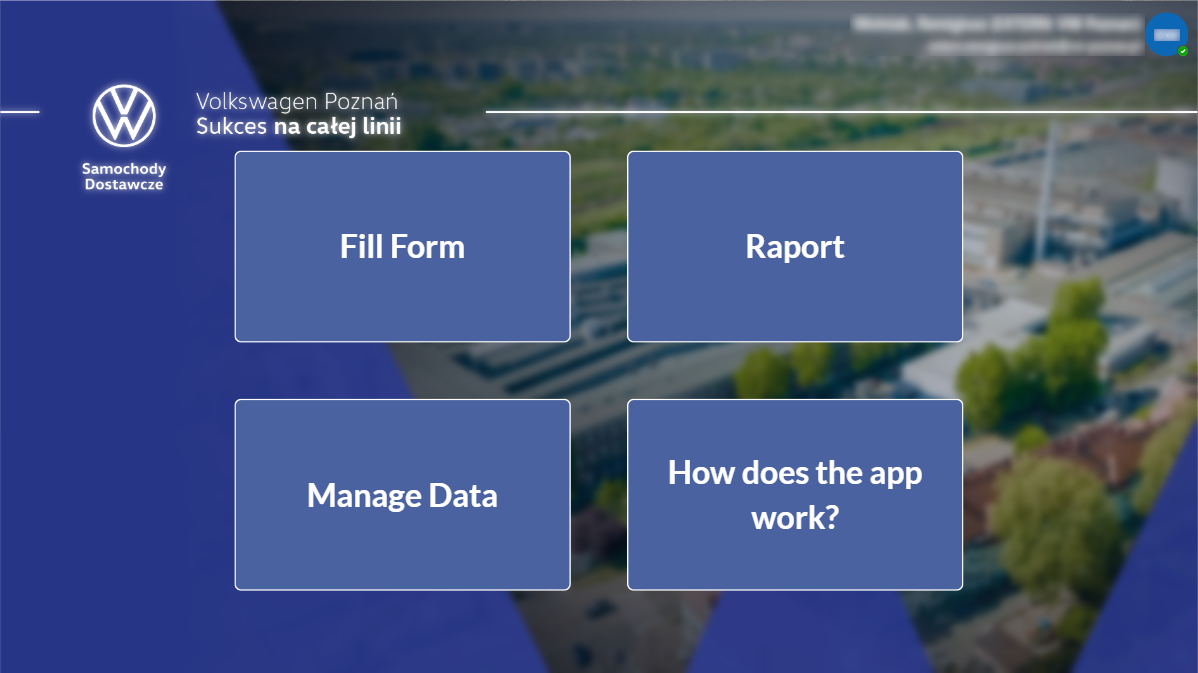
\includegraphics[width=0.9\textwidth]{figures/HomeScreen.png}
    \caption{Ekran startowy aplikacji} 
    \label{fig:homescreen}
\end{figure}

Dodatkowo, podczas uruchomienia aplikacji, pobierane są dane z list SharePointowych a następnie odpowiednio przetwarzane w celu płynnego wyświetlania ich w aplikacji. \\
Kod w języku \emph{Power Fx} wywoływany podczas uruchamiania aplikacji został przedstawiony w listingu \ref{lst:OnStartCode}.

\lstset{language=C,caption={Kod wywoływany podczas uruchamiania aplikacji},label=lst:OnStartCode}
\begin{lstlisting}[language=PowerFx]
 Set(varDownloadingData;true);;
 ClearCollect(colYears;{Value: Text(Now();"yyyy")-2};
 {Value: Text(Now();"yyyy")-1};
 {Value: Text(Now();"yyyy")+0};
 {Value: Text(Now();"yyyy")+1};
 {Value: Text(Now();"yyyy")+2}
 );;
 
 ClearCollect(colNumbers; {Value: 1};{Value: 2};{Value: 3};{Value: 4};{Value: 5});;
 
 Set(UserVar;UżytkownicyusługiOffice365.MyProfile());;
 
 // W OnStart aplikacji lub OnVisible ekranu
 ClearCollect(LocalServiceData; Lista_Uslug);;
 ClearCollect(LocalCostData; Lista_Kwot);;
 ClearCollect(LocalIndicationsData; Lista_Indykacji);;
 ClearCollect(
     MergedData;
     AddColumns(
         Lista_Uslug;
         Kwoty; LookUp(
             Lista_Kwot;
             Service_ID = Lista_Uslug[@Service_ID] &&
             Year = Max(Filter(Lista_Kwot; Service_ID = Lista_Uslug[@Service_ID]); Year)
         );
         Indykacje; LookUp(
             Lista_Indykacji;
             Service_ID = Lista_Uslug[@Service_ID] &&
             Year = Max(Filter(Lista_Indykacji; Service_ID = Lista_Uslug[@Service_ID]); Year) &&
             IndicationNo = Max(Filter(Lista_Indykacji; Service_ID = Lista_Uslug[@Service_ID] && Year = Max(Filter(Lista_Indykacji; Service_ID = Lista_Uslug[@Service_ID]); Year)); IndicationNo)
         )
     )
 );;
 Set(varDownloadingData;false);;
 \end{lstlisting}

 Na początku zmiennej \emph{varDownloadingData} przypisywana jest wartość \emph{true} za pomocą funkcji \emph{Set()}. Zmienna ta odpowiada za wyświetlenie wskaźnika ładowania oraz zablokowanie interfejsu użytkownika, aby uniemożliwić wprowadzanie zmian w trakcie ładowania danych.

Następnie funkcja \emph{ClearCollect()} tworzy kolekcję \emph{colYears}, która zawiera pięć elementów reprezentujących zakres lat od dwóch lat wstecz do dwóch lat naprzód. Podobnie powstaje kolekcja \emph{colNumbers}, zawierająca numery indykacji, które mogą być wykorzystywane w odpowiednich polach \emph{Dropdown}. Kolekcje te są pomocne przy budowie dynamicznego interfejsu użytkownika.

Za pomocą funkcji \emph{Set()} w kolejnej linii pobierane są informacje o obecnym użytkowniku i przypisywane do zmiennej \emph{UserVar}. Informacje te mogą być używane do personalizacji aplikacji lub kontroli dostępu.

Aplikacja tworzy następnie lokalne kopie trzech list danych (\emph{Lista\_Uslug}, \emph{Lista\_Kwot}, \emph{Lista\_Indykacji}) przy użyciu funkcji \emph{ClearCollect()}, co pozwala na szybsze filtrowanie i manipulację danymi podczas użytkowania aplikacji.

Kolejnym krokiem jest utworzenie kolekcji \emph{MergedData}, która łączy dane z list lokalnych kopii list. W tym celu zastosowano funkcję \emph{AddColumns()}, która dodaje dwie nowe kolumny: \emph{Kwoty} oraz \emph{Indykacje}. Dane w tych kolumnach są wyodrębniane przy użyciu funkcji \emph{LookUp()} oraz \emph{Filter()}, które umożliwiają filtrowanie i wyszukiwanie danych na podstawie określonych kryteriów.

Funkcja \emph{LookUp()} zwraca pierwszy rekord spełniający podane warunki, natomiast \emph{Filter()} generuje zbiór rekordów spełniających zadane kryteria. W analizowanym kodzie funkcje te są zagnieżdżone, co umożliwia precyzyjne wyodrębnienie danych z list na podstawie trzech kluczowych kryteriów:
\begin{itemize}
    \item \emph{Service\_ID} – identyfikator usługi,
    \item \emph{Year} – najwyższy rok dla pasującego identyfikatora usługi,
    \item \emph{IndicationNo} – maksymalny numer indykacji dla rekordów o zgodnym \emph{Service\_ID} i \emph{Year}.
\end{itemize}

Ostatecznie kolekcja \emph{MergedData} zawiera dane dla najnowszego roku i najwyższego numeru indykacji dla każdej usługi.

Na końcu zmiennej \emph{varDownloadingData} przypisywana jest wartość \emph{false}, co oznacza zakończenie procesu pobierania danych i gotowość aplikacji do użytku.

Lokalne kopie list (\emph{LocalServiceData}, \emph{LocalCostData}, \emph{LocalIndicationsData}) zostały utworzone w celu przyspieszenia działania mechanizmu filtrowania oraz zwiększenia efektywności podczas wyboru usług do edycji.




